

\TODO{TOTAL BUDGET: 14 pages}

\TODO{TENTATIVE TARGET PAGE BUDGET: 4 pages: state of art + vision; 2 pages: methodology overview; 5 pages:
WPs; 3 pages: ethics + risks}

\tableofcontents

\newpage

\newrefsection
\chapter{B2.a State-of-the-art and objectives}

\eu{(B2.a, B2.b: max 14 pages}
\eu{

Section a: State-of-the-art and objectives. Specify the proposal objectives in
the context of the state of the art in the research field. It should be clear
how and why the proposed work is important for the field, and what impact it
will have if successful, such as how it may open up new horizons or
opportunities for science, technology or scholarship. Specify any particularly
challenging or unconventional aspects of the proposal, including multi- or
inter-disciplinary aspects.


Section B: Methodology. Describe the proposed methodology in detail including
any key intermediate goals. Explain and justify the methodology in relation to
the state of the art. Highlight any intermediate stages where results may
require adjustments to the project planning. In case you ask that team members
are engaged by another host institution, their participation has to be fully
justified by the scientific added value they bring to the project.  }

%%%%%%%%%%%%%%%%%%%%%%%%%%%%%%%%%%%%%%%%%%%%%%%%%%%%%%%%%%%%%%%%%%%%%%%%%%%
%%%%%%%%%%%%%%%%%%%%%%%%%%%%%%%%%%%%%%%%%%%%%%%%%%%%%%%%%%%%%%%%%%%%%%%%%%%
%%%%%%%%%%%%%%%%%%%%%%%%%%%%%%%%%%%%%%%%%%%%%%%%%%%%%%%%%%%%%%%%%%%%%%%%%%%
\section{A. State-of-art and objectives}

%%%%%%%%%%%%%%%%%%%%%%%%%%%%%%%%%%%%%%%%%%%%%%%%%%%%%%%%%%%%%%%%%%%%%%%%%%%
\subsection{State-of-art: social representations for intelligent robots}

\TODO{copy-paste from the HRI paper}

The basic idea of \emph{social robots} refers to robots that are situated in a
human social environment. In this context, we expect social robots to exhibit
\emph{social awareness}, i.e. to appraise and maintain a model of the social
situation in which they are embedded. Depending on the role of the robot, this
might include understanding who is present, who is interacting with whom, which
are the resulting groups,  what are the in-group roles,  etc.

Social awareness, as a socio-cognitive skill, is essential for the robot to e.g.
act in a context-sensitive manner; reason and apply social norms (for instance,
do not navigate in the middle of a group, or do not suddenly interrupt a
conversation); or create proactive social agents (in order to acknowledge and
respond to a human who would like to engage with the robot, the robot must first
adequately model and recognise the corresponding social situation).

\emph{Social situations} have indeed been an important object of study in social
psychology for a long time~\cite{argyle1981social}, with, for instance, the
following definition by Garbett~\cite{garbett1970analysis}: \emph{a social
situation is a temporally and spatially bounded series of events abstracted by
the observer from the on-going flow of social life}. When specifically looking
at artificial agents like robots, their level of social cognition depends on
their ability to identify and interpret the world surrounding
them~\cite{szczepanowski2017computational}, and in particular, correctly interpret
transactions of social signals -- specific events in which an agent performs a
social action aimed at another agent~\cite{pantic2011social}. This process is known as
\textit{situational awareness}, of which Endsley~\cite{endsley1995theory} defines
three levels:\emph{perception}, \emph{interpretation}, and \emph{evaluation}.

While the \emph{perception} of social signal has been studied in depth in the
HRI community (for instance,~\cite{pantic2011social}), and the \emph{evaluation} of
the social situation is usually handled as an aspect of the robot's decision
making, the \emph{interpretation} of social situations is a difficult problem.
It requires to build and maintain a task-appropriate model of the situations,
and represent it in such a way that a machine can reason about it.
\emph{Embeddings} are such representations.


\subsubsection{Embeddings}

In the context of machine learning, we refer to an \emph{embedding} as a
real-valued vector representation of a typically much higher dimensionality
input. In other words, a representation that encodes high-dimensionality input
(for instance, an image) into a lower-dimensional space. Critically, embeddings
are trained to encode the relationships and semantic nuances that might exist in
the original input space. For instance, two pictures of the same face
transformed with an embedding tuned for facial recognition would yield two
vectors that are similar to each other (i.e., close to each other for a given
metric, usually the cosine distance). As such, the process of embedding not only
condenses high-dimensional information into a more manageable form but also
captures latent associations that might otherwise remain
obscured~\cite{bengio2009learning}.

Unsurprisingly, the training of compact yet semantically-rich embeddings has
been a very active research topic over the last two decades, yielding
exceptional results in machine learning, where the (otherwise high)
dimensionality of real-world percepts might turn common machine learning
tasks like classification or prediction intractable.

While research on embeddings initially focused on data that would intuitively
lend itself well to mathematical transformations (for instance, reducing the
dimensionality of an image, represented as an array of pixel intensities, or
processing sound), it has since then been discovered that many constructs --
physical or not -- can also be \emph{embedded} in a low-dimension numerical
space, while preserving many of their semantics. One of the landmark
achievements in that regard is the work published in 2013 by Mikolov et al. --
themselves building on previous work spanning another decade.  They showed that
embeddings can be computed for \emph{words}, also encoding some of their
semantic meaning~\cite{mikolov2013efficient}, with the famous example of
\emph{embedding(`king') - embedding(`man') + embedding(`woman') $\approx$
embedding(`queen')}. Effectively, a conceptual equivalence of terms, involving
semantics related to gender and social role could be transformed into simple
mathematical additions and subtractions.

This outcome ushered in a decade of intense research on text representation,
ultimately resulting in the current Large Language Models (LLM) like GPT or
Llama2.  Most of the recent progress has been enabled by the discovery in 2017
of the attention-based \emph{Transformers}~\cite{vaswani2017attention} neural
network structure, which brought a boost to the research on natural language
procesing with, for instance, BERT~\cite{devlin2019bert} in 2019 and the family
of GPT models~\cite{wolf2020transformers} in 2020.  These large models
are pre-trained on massive text corpora and are typically used for token
prediction (the pre-trained network is fed with a text context, and predicts the
next tokens).  Importantly for this work, these very large pre-trained networks
can also be used to compute text-level embeddings, representing a short text as
a numerical vector~\cite{reimers2019sentencebert,muennighoff2022sgpt}. The
resulting embeddings can be then used to measure text-relatedness for instance,
as in the BEIR benchmark~\cite{thakur2021beir}.

\subsection{Key insight}

Combining the above concepts of social situations and text embeddings, we introduce in
this paper the idea of \emph{social embeddings}. A \emph{social embedding} is a
compact, real-valued numerical representation (a vector) of a social
situation, as experienced by an agent immersed in that social environment.
Following the general idea of embeddings, social embeddings are designed
to encode the \emph{semantics} of the social situation currently experienced by
the agent, facilitating the interpretation of the situation. For instance, it
could make it straightforward to compare two social situation by simply
measuring how similar the two corresponding embeddings are.

The key insight to construct these embeddings is to exploit the social knowledge
already encoded in the latent space of large language models. We do so by
automatically generating a textual description of the social environment of the
robot (using regular perception routines), and by transforming this
description into a text embedding via a large language model. By doing so, we
effectively construct an \emph{embedding}, i.e., a projection, of the social
space into a machine-friendly numerical space.

This article is a first investigation of this idea. In the following sections,
we start the exploration of the design space of social embeddings by presenting
a simple algorithm to generate scene descriptions and derive embeddings; we
analyse and discuss several key characteristics and parameters of the derived
embeddings -- like their application as a quantitative \emph{social distance};
and we discuss several promising directions for follow-up research.


\subsection{Motivating example}

\begin{figure}[ht!]
     \centering
     \begin{subfigure}[b]{0.3\columnwidth}
         \centering
         \includegraphics[width=\textwidth]{figs/sit1.png}
         \caption{``I'm chatting with one person; another group of two people
         are discussing on the side."}
         % short code: eJxtUktqwzAQvYrR2hEjaUafLgvd9ADtIoRgUzUxcW1I3LSh9O4dKQlYpsLYwzPzfvZ6Lb5FXYlLuk37ODVpOGfsfAWb/tANuzTGYdfs4tv2q5v2YlNXa3Ec23HiVystwcD8aAZBWh2KU1dwv96b/hSZg3nE00fXJzHecCY/vC/YGFTWS09OKVCorAV3J5qOn3ee167vmQbYjKbF/kpJS2oOJ5DYuCVPzBeItPNZHcpt0DqTgsZ5GLSuUH/pxj7e2lBsmEPUFXmpA/sGYwADav9f/udmiCJtBHSUrarCabaKXhpr0YK1BplTJU/ocVFwaj0sw8/FHsc2d4ShiONcNm7CsiNljHREbB88AtDtC/FUdASIV9y4Oa1Fmsmz/o84xThs24t4qG7/z+/mD6BekW4=
         % generated description: Bob is not far from me; Emily is close to me; Emily and I are looking at each other; Bob and Will are looking at each other; Will is talking; Emily is talking; Bob is looking at me

         \label{soc_sit_a}
     \end{subfigure}
     \begin{subfigure}[b]{0.3\columnwidth}
         \centering
         \includegraphics[width=\textwidth]{figs/sit2.png}
         \caption{``In front of me, three people chatting together;
         someone is walking towards me."}
         % short-code: eJx1UttOwzAM/ZUqzyOKnYsTHpF44QPgoZqmVoStorTSVgYT4t9x0g41SFhtY53E59g5rWvxKTaVuKTPdIhTk5Jzxs4z2PSv3bBPaRz2zT4+7z666SC2m6oWx7EdJ966Qam0WgcyqKTDUMSmUtfnpelPkTmYR9y/dX0S4wqDuKYByyhIcilJhVIpXwgpynUMr4V8oFLiqet7VgCpAxpw1/AmV4OCdTW5pEpOKuO0tY4MEzqfj/Lq9W+gnes1/Jlzrf3YjX1M14TSmHkgQ0CcWS8xeEtKa2WCQZ8m1FTMBwlzEMz/Ag/NEEU+5mnmR4K0opJondEEPAcGXO4KCq6wmKXQFQ6mVtcqd2M7i5T9YbYfgXsCa2W6HGLf+DV24S0NA3/toqDRbMV0fM9qLPclTjEOu/YibqvlP/ve/gBPLpnY
         % generated desc: Bob is not far from me; Will is walking towards me; Bob is talking; Will and I are looking at each other; Will is not far from me; Bob is looking at Emily; Bob is looking at me
         \label{soc_sit_b}
     \end{subfigure}
     \begin{subfigure}[b]{0.3\columnwidth}
         \centering
         \includegraphics[width=\textwidth]{figs/sit3.png}
         \caption{``A group of two people are chatting;
         someone is walking towards me."}
         % short-code: eJxtkNFuwyAMRX8l4jlBYHCAvu8XtoeoqhKVpag0kRLWrZr27wPWTElVC4FlfM81NA35ImVBbmkLJxvalFxz7fpXbP3ZDX1K7dC3vT0ePl04kX1ZNGQauzHEqwqorOPBqEG2DigLtqz31s82qqKSvFycT3hGgZt1KMwYhE1VrzBh+lgob877COFUiE27yQwZVRVXinIjajBKauBc6WfjvLrR25DnQSkfURCHVLh9FUekTHEE1LVEoZXInnqrTmZUwqP43zp6f5PZ2uHQ3ciuuP/nz/4XWRhgxw==
         % generated desc: Emily and Will are looking at each other; Violet is not far from me; Violet is looking at me; Violet is walking towards me; Will and I are looking at each other; Will is not far from me; Emily is talking
         \label{soc_sit_c}
     \end{subfigure}

        \caption{Three simple social situations, described
        from the perspective of the yellow agent (arrows indicate direction and
        magnitude of motion).}
        \label{fig:social-situations}
\end{figure}


Figure~\ref{fig:social-situations} shows three schematic social situations,
described from the egocentric perspective of the yellow character. In
Figure~\ref{soc_sit_a}, the character is engaged with one person, and another
group of two people are chatting; in Figure~\ref{soc_sit_b}, no one is
interacting directly with the character (but someone is walking towards
her/him), and three people seem to be chatting
together on the side; similarly in Figure~\ref{soc_sit_c}, someone is walking
towards the character, with another group of two people chatting together.

From the perspective of the yellow person the social situations depicted in \ref{soc_sit_b} and \ref{soc_sit_c}
are more similar: in both cases, the person is not actively engaged in an
interaction yet, but someone seems about to do so. However, a cursory
look at the scene could lead to think that \ref{soc_sit_a} and
\ref{soc_sit_b} are closer to each other, since they both involve more people
than \ref{soc_sit_c}, and most people seem located at the left of the main
character.

Accordingly, social embeddings are to be designed so that the situations from
Figures~\ref{soc_sit_b} and \ref{soc_sit_c} are closer in the embedding space
than situations~\ref{soc_sit_a} and \ref{soc_sit_b}: by doing so, a robot could
correctly compute similarities between social scenes, and e.g. recognise a
situation as similar to one it would have previously experienced.


%%%%%%%%%%%%%%%%%%%%%%%%%%%%%%%%%%%%%%%%%%%%%%%%%%%%%%%%%%%%%%%%%%%%%%%%%%%
\subsection{Objectives of \project}

\TODO{currently copy-paste of part B1}
%\project is built around three axes: a basic research programme; an experimental
%programme that looks specifically at the application of social embeddings to
%social robotics; and, running in parallel to those first two axes, a scientific
%investigation of the ethical dimension of social embeddings.

At the basic research level, \project targets two overarching research goals:

(1) to build compact, yet semantics-preserving, embeddings to represent
arbitrary social environments; and to fully characterize these embeddings,
including their latent semantics. I translate this first goal into objective
{\bf O1}: To \textbf{construct and characterize the fundamental
properties of social embeddings}.

(2) to precisely \textbf{define and implement the socio-cognitive skill of \emph{social awareness} enabled
by social embeddings}, and demonstrate it on social robots. I split this second
goal into three specific objectives: \emph{social appraisal}, \emph{social
learning}, \emph{social prediction}.

% 3 objectives:
%- appraise social situations, also taking into account the social context
%- learn socially-appropriate behaviours
%- anticipate future social states


\begin{enumerate}[label=\textbf{O\arabic*}]
    \setcounter{enumi}{1}
    \item \label{T5} To use social embeddings to \textbf{automatically appraise
        social situations}, taking into account their \textbf{context}. Using
        a set of prototypical reference situations, social embeddings
        can be used to relate the current social situation to known ones.
        Besides, because social embeddings lend themselves to jointly encode
        social context by simply attaching context descriptions, the appraisal
        of the social situation can be made \emph{context-aware};

    \item \label{T4} To \textbf{learn socially-appropriate behaviours} by using
        social embeddings as an additional input feature to existing behaviour
        generation algorithms like Generative Adversarial
        Networks~\cite{marmpena2019generating,suguitan2020moveae}; and by
        augmenting existing interactive machine learning techniques (`user
        in-the-loop' social learning, that I pioneered in social
        robotics~\cite{senft2017supervised, winkle2020couch,winkle2021leador})
        with representations of the social environment;

    \item \label{T2} To use social embeddings to model \textbf{social dynamics}
        by characterizing the trajectories of on-going social situations in the
        embedding space. I will look in particular into trajectories'
        \emph{discontinuties}, that might represent unexpected changes of social
        dynamics, and trajectories' extrapolations, that might represent
        \textbf{social situation \emph{predictions}}.

\end{enumerate}


\subsection{Basic research objectives}

\subsection{Empirical research objectives}


%%%%%%%%%%%%%%%%%%%%%%%%%%%%%%%%%%%%%%%%%%%%%%%%%%%%%%%%%%%%%%%%%%%%%%%%%%%
\subsection{Importance and impact of the project}

\TODO{rework}

Academically, the \project project represents a timely combination of
very recent advances in supervised machine learning for social robot
behaviour with a creative and interdisciplinary approach to the design
and automation of social robot behaviour. 
We will publish \project results in interdisciplinary and high-profile
discipline-specific journals (eg. Science Robotics; Frontiers in AI and
Robotics; Transaction in Human-Robot Interaction) and conferences (eg. AAAI,
HRI, RSS).

The dataset of social behaviours and social signals we will create and
distribute represents a one-in-a-kind resource for the human robot
interaction community, and the human data collection will be
transferable to research in other domains such as human-computer
interaction.

As \project will be deployed in a living lab environment, there is
significant scope for public outreach/engagement and media coverage,
which we will work with the BRL's media manager to maximise.


\project aims at building unique European capacity to assert leadership in this
domain, and, beyond the specific deliverables of this 5-years project,
establishing the PI as a world-leader in goal-driven, socially-responsible
robotics.


%%%%%%%%%%%%%%%%%%%%%%%%%%%%%%%%%%%%%%%%%%%%%%%%%%%%%%%%%%%%%%%%%%%%%%%%%%%
\subsection{Interdiscplinary nature of the project}

\TODO{rework}

\project paves the way for a better understanding of the societal challenges
raised by the rapid development of AI and robotics. Grounded in both the
psycho-social literature of human cognition, and the latest technological
advances in artificial cognition and human-robot interaction, the project
delivers major conceptual, technical and experimental contributions across
several fields: AI, ethics, sociology of technology, intelligent robotics,
learning technology. As such, \textbf{\project builds bridges across
multiple disciplinary boundaries}.

\project delivers this programme by building on a range of multidisciplinary
methods, including user-centered design; ethnographic and sociological
investigation; expressive non-verbal communication, including dance and
puppetering; embodied cognition; symbolic AI; neural
nets and sub-symbolic AI; interactive machine learning.

Accordingly, the project builds on a \textbf{strong interdisciplinary team}: the
post-docs directly recruited on \project will have backgrounds in sociology of
technology (PD1), cognitive modeling (PD2), machine learning (PD3), cognitive
robotics (PD4). Additional expertise will be recruited to provide specific
support: the \project Ethics Advisory Board will contribute expertise to guide
the work on ethics; Dr. Newbutt will provide expertise in learning technologies
and cognitive impairment; Dr. Meckin will provide expertise in sound-based
expressive communication; the WeTheCurious science centre will provide training
in large-scale public engagement; the Bristol Children's hospital will bring the
required expertise in working with young patients; the RustySquid company will
provide expertise in expressive arts and puppetering.



%%%%%%%%%%%%%%%%%%%%%%%%%%%%%%%%%%%%%%%%%%%%%%%%%%%%%%%%%%%%%%%%%%%%%%%%%%%
%%%%%%%%%%%%%%%%%%%%%%%%%%%%%%%%%%%%%%%%%%%%%%%%%%%%%%%%%%%%%%%%%%%%%%%%%%%
%%%%%%%%%%%%%%%%%%%%%%%%%%%%%%%%%%%%%%%%%%%%%%%%%%%%%%%%%%%%%%%%%%%%%%%%%%%
\newpage
\section{B. Methodology}

%%%%%%%%%%%%%%%%%%%%%%%%%%%%%%%%%%%%%%%%%%%%%%%%%%%%%%%%%%%%%%%%%%%%%%%%%%%
\subsection{Overview of \project methodology}

\TODO{section to fully update}

The four research questions previously listed are addressed across five
work-packages: \textbf{WP1} is dedicated to the conceptual framing of the
project (R1) and the identification of interaction principles; \textbf{WP2}
extracts from these principles the set of requirements in term of
socio-cognitive capabilities for the robot (R3), and implement them; in parallel
to WP2,  \textbf{WP3} looks at how social robots can generate congruent social
behaviours (R3); \textbf{WP4} transposes the conceptual framework of WP1 into a
principled cognitive architecture and integrates together the cognitive
functions of WP2 and WP3 (R2);and \textbf{WP5} organises the experimental
fieldwork that demonstrates the \project approach in ambitious and complementary
real-world situations (R4).



\begin{figure}[h!]
\centering
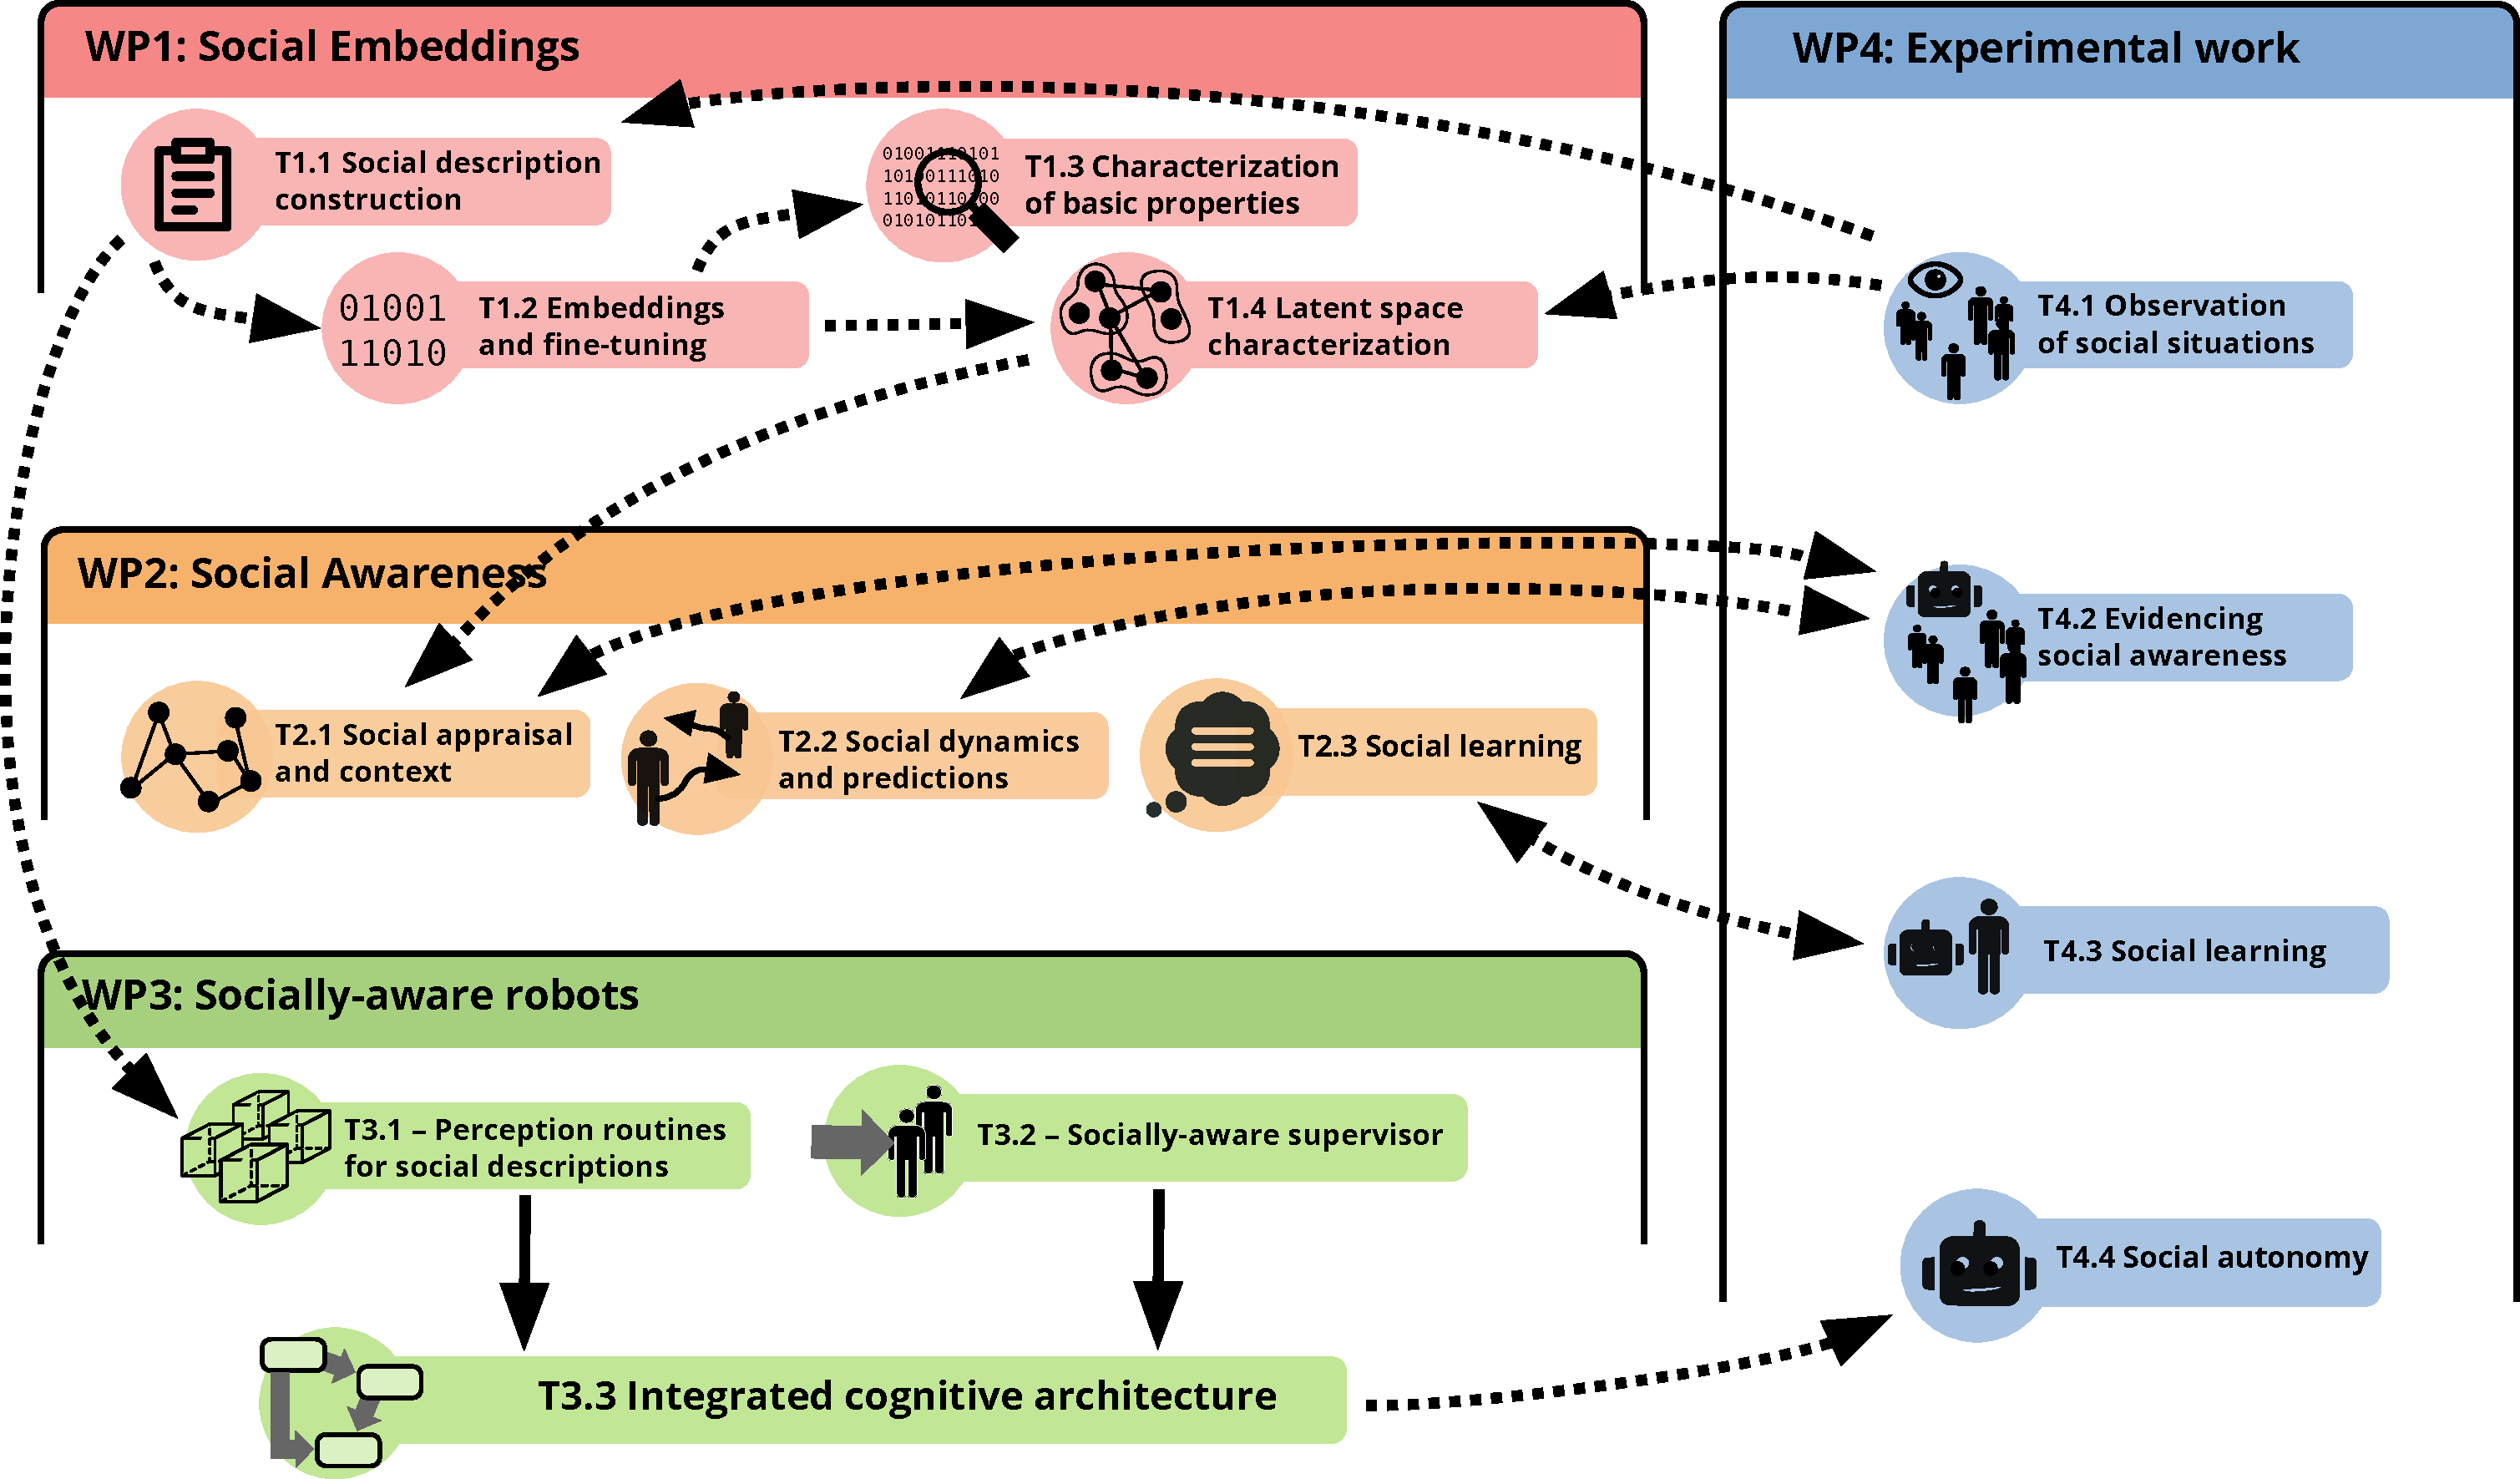
\includegraphics[width=\linewidth]{figs/wps}
\caption{Overview of the workpackages and tasks, and tasks inter-relations.}
\label{fig:wps}
\end{figure}

More specifically, Figure~\ref{fig:wps} gives an overview of the project
workpackages, and their interrelations. Fieldwork plays a central role in the
project, and appears in the centre of the figure. The first important field
deployment is a one-year experiment, taking place at the Bristol science centre
(T1.1). This `public-in-the-loop' experiment is analysed and lead to the
definition of core interaction principles (T1.2). These are in turn translated
into algorithmic models, guiding the social teleology of the cognitive
architecture (T4.1).

This first experiment is immediately followed by two other long-term
experimental deployments: a one-year deployment in one of Bristol's Special
Education Need (SEN) school (T5.1), followed by a one-year deployment at
Bristol's Children's hospital (T5.2). These two additional experiments are both
inputs for WP2 and WP3, and demonstrator for the robot socio-cognitive
architecture (WP4).

Specifically, workpackage WP2 research, develop, and integrate all the components
pertaining to the assessment of the spatio-temporal and social environment of
the robot. Reference interaction situations and the data required to support
this workpackage is directly drawn from the experimental fieldwork that will
take place at the same time in WP1 and WP5. The perceptual capabilities
delivered by WP2 are continuously integrated into the robot's cognitive
architecture (T4.3), iteratively improving the socio-cognitive performances of
the robot.

Workpackage WP3 looks into behaviour generation using machine learning (T3.2)
and non-verbal affective modalities (T3.3). T3.2 is data-intensive, and will use
datasets acquired during the field deployments (T1.1, T5.1, T5.2), as well as
lab-recorded dataset of social interactions. Similar to WP2, the capabilities
built in WP3 are integrated in the robot architecture in T4.3.

In addition to the integration of WP2 and WP3 capabilities, WP4 is also
researching and developing the socio-cognitive drives of the architecture. They
come both from T1.2 (as previously mentioned), and
human-in-the-loop/public-in-the-loop machine learning (T4.2). T4.2, in
particular, is tighly connected to the experimental fieldwork, where the
learning-from-end-users take place.

\subsubsection{Integration sprints}

\project is a complex project, with numerous interdependencies between tasks.
To ensure the interdependencies are properly understood, and support effective
integration of the outputs of each workpackage, I will organise every 6 months
\textbf{integration sprints} (see Gantt diagram). Integration sprints are
one-week long integration retreat during which the whole \project team gather
and work together to effectively implement and test on the robot the different
components. In addition to providing regular `check points' for the projects,
they also set a stable schedule to deliver project components.

This methodology was used by the PI in  several previous projects (FP7 CHRIS
project, H2020 SPRING for instance), and had proved to be of great value to
ensure project-wide cohesion and steady progress.

The three integration sprints taking place before the beginning of the
experimental deployments (display as orange circles on the Gantt chart) are of
particular importance, and will be extended to ten days.


\subsubsection{Gantt chart}

%\begin{landscape}
\begin{figure}[!ht]
\resizebox{\linewidth}{!}{
    %%%%%%%%%%%%%%%%%
%%
%% Task dependencies
%%
%% Task...        depends on Task...
%% T1.3           T1.1
%% T1.3           T1.2
%% T1.2           T2.2 (user interface)
%% T3.3           T2.3
%%

\definecolor{barcolor}{RGB}{153,204,254}
\definecolor{linkred}{RGB}{165,0,33}
%\renewcommand\sfdefault{phv}
%\renewcommand\mddefault{mc}
%\renewcommand\bfdefault{bc}
\setganttlinklabel{s-s}{START-TO-START}
\setganttlinklabel{f-s}{}
\setganttlinklabel{f-f}{FINISH-TO-FINISH}

%\begin{sidewaysfigure}[!ht]
\begin{figure}[!ht]

%\sffamily
\begin{ganttchart}[
        canvas/.append style={fill=none, draw=black!5, line width=.75pt},
        hgrid style/.style={draw=black!5, line width=.75pt},
        vgrid={*1{draw=black!5, line width=.75pt}},
        %vgrid={*1{black}, *{11}{black!5}}, % doesnt work for some reason
        x unit=.35cm,
        y unit chart=.65cm,
        time slot format=isodate-yearmonth,
        time slot unit=month, % pgfgantt >= 5.0
        %compress calendar, % pgfgantt < 5.0 => overleaf
        title/.style={draw=none, fill=none},
        title label font=\bfseries\footnotesize,
        %title label node/.append style={below=7pt},
        include title in canvas=false,
        bar label font=\mdseries\small\color{black!70},
        %bar label node/.append style={left=2cm},
        bar/.append style={draw=none, fill=barcolor!50},
        bar progress label font=\mdseries\footnotesize\color{black!70},
        group/.append style={fill=barcolor},
        group incomplete/.append style={fill=black},
        group left shift=0,
        group right shift=0,
        group height=.5,
        group peaks tip position=0,
        group label node/.append style={left=.6cm},
        group progress label font=\bfseries\small,
        link/.style={-latex, line width=1.5pt, linkred},
        link label font=\scriptsize\bfseries,
        link label node/.append style={below left=-2pt and 0pt,
        milestone/.append style={circle},
        milestone inline label node/.append style={left=5mm}}
    ]{2021-01}{2025-12}
    
        %\gantttitle[
        %    title label node/.append style={below left=7pt and -3pt}
        %]{Month:\quad1}{1}
        \gantttitlecalendar{year, month} \\
        %\gantttitlelist{0,5,...,60}{1} \\
        %% WP1
        \ganttgroup[]{WP1 \wpOneShort}{2021-01}{2023-12} \\
            \ganttbar[name=WP11]{\textbf{1.1} Conceptual framing \& ethics}{2021-01}{2023-12} \\
            \ganttbar[name=WP12prep,inline,bar/.append style={fill=gray!20}]{preparation}{2021-07}{2021-12}
            \ganttbar[name=WP12exp,inline]{WeTheCurious experiment}{2022-01}{2022-12}
            \ganttbar[name=WP12]{\textbf{1.2} Principles of r-HHI}{2023-01}{2023-06} \\

        %\ganttlink[link type=f-s]{WBS1A}{WBS1B}

        %% WP2
        \definecolor{barcolor}{RGB}{153,2,254}
        \ganttgroup[]{WP2 \wpTwoShort}{2021-01}{2024-12} \\
            \ganttbar[name=WP21]{\textbf{2.1} Situation assessment}{2021-01}{2022-06} \\
            \ganttbar[name=WP22]{\textbf{2.2} Social dynamics}{2022-01}{2023-12} \\
            \ganttbar[name=WP23]{\textbf{2.3} Group dynamics}{2024-01}{2024-12} \\
            \ganttbar[name=WP24]{\textbf{2.4} Social situation assessment}{2022-07}{2024-12} \\

        %\ganttlink[link type=f-s]{WP21}{WP24}
        %\ganttlink[link type=f-s]{WP22}{WP23}

        %% WP3
        \definecolor{barcolor}{RGB}{50,220,134}
        \ganttgroup[]{WP3 \wpThreeShort}{2021-01}{2025-12} \\
            \ganttbar[name=WP31]{\textbf{3.1} Social teleology}{2023-01}{2024-12} \\
            \ganttbar[name=WP32]{\textbf{3.2} Human-in-the-loop policy learning}{2021-07}{2025-06} \\
            \ganttbar[name=WP33]{\textbf{3.3} Integrated cognitive architecture}{2021-01}{2025-06} \\

        %\ganttlink[link type=f-s]{WP12}{WP32}

        %% WP4
        \definecolor{barcolor}{RGB}{244,50,20}
        \ganttgroup[]{WP4 \wpFourShort}{2022-01}{2025-12} \\
            \ganttbar[name=WP41]{\textbf{4.1} Behaviours baselining}{2022-01}{2022-12} \\
            \ganttbar[name=WP42]{\textbf{4.2} Generative behaviours}{2023-01}{2023-12} \\
            \ganttbar[name=WP43]{\textbf{4.3} Non-verbal behaviours}{2023-07}{2025-12} \\


        %% WP5
        \definecolor{barcolor}{RGB}{234,200,20}
        \ganttgroup[]{WP5 \wpFiveShort}{2022-07}{2025-12} \\
            \ganttbar[name=WP51prep,inline,bar/.append style={fill=gray!20}]{preparation}{2022-07}{2022-12}
            \ganttbar[name=WP51]{\textbf{5.1} SEN schools experiment}{2023-01}{2023-12} 
            \ganttbar[name=WP51expl,inline,bar/.append style={fill=gray!20}]{analysis}{2024-01}{2024-06} \\
            \ganttbar[name=WP52prep,inline,bar/.append style={fill=gray!20}]{preparation}{2024-01}{2024-06}
            \ganttbar[name=WP52]{\textbf{5.2} children hospital experiment}{2024-07}{2025-06}
            \ganttbar[name=WP52expl,inline,bar/.append style={fill=gray!20}]{analysis}{2025-07}{2025-12} \\

        %\ganttlink[link type=f-s]{WP41}{WP51}


        %\ganttlink[link type=f-s]{WBS1B}{WBS1C}
        %\ganttlink[link type=f-f,link label node/.append style=left]{WBS1C}{WBS1D}

        \ganttmilestone{\bf\sc Integration sprints}{2021-06}
        \ganttmilestone[milestone/.append style={fill=orange, circle}]{}{2021-11}
        \ganttmilestone{}{2022-06}
        \ganttmilestone[milestone/.append style={fill=orange, circle}]{}{2022-11}
        \ganttmilestone{}{2023-06}
        \ganttmilestone{}{2023-12}
        \ganttmilestone[milestone/.append style={fill=orange, circle}]{}{2024-05}
        \ganttmilestone{}{2024-12}


        % separate years
        \ganttvrule[vrule/.append style={gray, dotted, thin}]{}{2021-12}
        \ganttvrule[vrule/.append style={gray, dotted, thin}]{}{2022-12}
        \ganttvrule[vrule/.append style={gray, dotted, thin}]{}{2023-12}
        \ganttvrule[vrule/.append style={gray, dotted, thin}]{}{2024-12}


        \ganttvrule{start @WeTheCurious}{2021-12}
        \ganttvrule{start @SEN school}{2022-12}
        \ganttvrule{start @Children hospital}{2024-06}

\end{ganttchart}

%\end{sidewaysfigure}
\end{figure}

}
\end{figure}
%\end{landscape}


\subsubsection{Project's milestones}

\begin{table}[h!]
    \centering
\begin{tabular}{@{}lccccccr@{}}
\toprule
\textit{\textbf{}}              & \textbf{Y1} & \textbf{Y2} & \textbf{Y3} & \textbf{Y4} & \textbf{Y5} \\ \midrule
\textit{MS1:...} &   & x  &    &   &    &  &   \\ 
\textit{MS2:...} &   &    & x  &   &    &  &   \\ 
\textit{MS3:...} &   &    &    & x &    &  &   \\ 
\textit{MS4:...} &   &    &    &   & x  &  &   \\ \bottomrule
\end{tabular}
    \caption{Project's milestones}
    \label{milestones}
\end{table}

\subsubsection{Engineering methodology}

\TODO{useful?}

Detail use of:
\begin{itemize}
    \item use of ROS2
    \item coding guidelines enforced with linters
    \item CI/CD for automatic code testing
    \item integration testing using DOcker/Docker compose
\end{itemize}

%%%%%%%%%%%%%%%%%%%%%%%%%%%%%%%%%%%%%%%%%%%%%%%%%%%%%%%%%%%%%%%%%%%%%%%%%%%
\subsection{Expertise and Research team}
\label{research-team}

My expertise is primarily centered on cognitive robotics and human-robot social
interaction. My expertise in this field covers a broad spectrum, from basic
research in robotics (for
instance~\cite{lemaignan2014dynamics,lemaignan2015mutual}) and data-driven
socio-psychology
(including~\cite{lemaignan2014cognitive,irfan2018social,winkle2019effective,bartlett2019what}),
to technical contributions (for instance~\cite{lemaignan2010oro,
lemaignan2017artificial, lemaignan2018underworlds}), to extensive experimental
work (see below; for instance~\cite{hood2015cowriter,winkle2020couch,
lemaignan2022social}).

Over the last 4 years, I have re-focalised my work on \emph{data-driven HRI},
contributing several new large datasets of social
interactions~\cite{lemaignan2018pinsoro,sallami2020unexpected,webb2023sogrin},
developing new data analysis
techniques~\cite{bartlett2019what,webb2022measuring}, and demonstrating with my
students new applications of interactive machine learning to social
interactions~\cite{senft2016sparc,winkle2020couch,winkle2021leador}.  In
parallel, I progressively matured the idea of computing compact
\emph{embeddings} of social situations, until I recently published a first
breakthrough in that direction~\cite{lemaignan2024social} (to appear at IEEE/ACM
HRI'24). This ERC project is directly born from this multi-year endeavour
towards data-driven social sciences applied to embodied AI systems, and aims at
significantly accelerate research in this direction.

In particular, \project is the opportunity to gather an interdisciplinary team
of academics that would effectively complement my expertise, and ensure the
feasibility of the project.

Specifically, I intend to recruit:

\begin{itemize}

    \item  two researchers with expertise in data-driven
        socio-psychology (one senior post-doc PD1, one PhD student PHD1); these
        researchers will directly contribute to the human data acquisition,
        the interpretation of social embeddings in term of social situations,
        and the experimental work;

    \item two researchers with expertise in deep machine learning and large
        language models (one senior post-doc PD2, one PhD student PHD2); these
        researchers will contribute to the core implementation of social
        embeddings, including language model fine-tuning, as well as the
        analysis of the embedding space topology;

    \item one research in cognitive robotics (PhD student, PHD3); this
        researcher will focus on the effective integration of social
        embeddings into a larger cognitive architecture for social robots, able
        to autonomously drive interactions;

    \item one researcher in ethics of technology (post-doc
        level PD3); this researcher will lead the work on understanding social
        embeddings in terms of ethical and responsible research.
\end{itemize}

Table~\ref{time-allocation-team} provides an overview of the time allocation per
members of the team, over the course of the project.

\begin{table}[h!]
    \centering
\begin{tabular}{@{}lccccccr@{}}
\toprule
\textit{\textbf{}}              & \textbf{Y1} & \textbf{Y2} & \textbf{Y3} & \textbf{Y4} & \textbf{Y5} &  & \textbf{Total months} \\ \midrule
\textit{Séverin Lemaignan (PI)} & 1         & 1         & 1         & 1
    & 1         &  & 60                    \\ \midrule
\textit{Post-doc 1 (WP1)}       & 1           & 1           & 1           &             &             &  & 36                    \\
\textit{Post-doc 2 (WP2)}       & 1           & 1           & 1           & 1           &             &  & 48                    \\
\textit{Post-doc 3 (WP3)}       &             & 1           & 1           & 1           & 1           &  & 48                    \\
\textit{Post-doc 4 (WP3, WP5)}  & 1           & 1           & 1           & 1           & 1           &  & 60                    \\
\textit{PhD 1 (WP3, WP5)}       &             & 1           & 1           & 1           & 0.5         &  & 42                    \\ \bottomrule
\end{tabular}
    \caption{Full-time equivalent for the research team members\TODO{to update}}
    \label{time-allocation-team}
\end{table}


In addition, the host institution (INRIA Grenoble) will provide extensive
additional expertise on machine learning applied to robotics. I will specifically build on
my already established collaboration with Dr. Xavier Almeida-Pineda, head of the
RobotLearn research group. Dr. Almeida-Pineda is the coordinator of the EU H2020
SPRING project on social robotics for geriatric care, on which I collaborated
for the past two years.

Additional expertise, as well as access to one of my main experimental
environment, will be provided through a collaboration with Paris' public
hospitals (APHP) and specifically, with Dr. Maribel Pino, head of research at
Paris' Broca geriatrics hospital (Dr. Pino has extensive experience running
studies with social robots on the hospital' premisses).


%%%%%%%%%%%%%%%%%%%%%%%%%%%%%%%%%%%%%%%%%%%%%%%%%%%%%%%%%%%%%%%%%%%%%%%%%%%
\subsection{Workpackages}

\subsubsection{WP1: \textbf{\wpOne}}

WP1 addresses Objective \textbf{O1}. I will first systematically investigate the
three steps of social embeddings construction, and then characterize the
resulting embeddings.

Social embeddings construction requires first to extract descriptors, then to
build complete textual descriptions, and finally to embed these descriptions.  I
will extract basic social descriptors using the ROS4HRI social perception
approach, as it formalize a multi-modal model of humans~\cite{lemaignan2022ros},
and run in real-time on current robots. I will augment these basic descriptors
with more complex percepts, including (1) descriptors of human-objects
interactions (HOI), using transformer-based techniques
like~\cite{iftekhar2022what} ; (2) affective
descriptors~\cite{vinciarelli2009social}, using e.g. facial expressions based on
facial action units classification~\cite{martinez2019automatic}; (3) group-level
interactions, including $f$-formations~\cite{setti2015fformation}, and group
activity recognition, using deep convolutional graph techniques like
ARG~\cite{wu2019learning}.

%(3) a novel contextual model of
%attention~\cite{ferrini2024percepts} that allows fine-grained assessment of what
%the person around the robot are focusing on.

The generation of textual descriptions consists in both the combination of
descriptors into textual \emph{snapshots} of the social environment at a
specific time, and the combination of these snapshots over time, to build a
textual description of complete situations with a time horizon of 10s to
25s~\cite{netanyahu2021phase}. I will initially build snapshots using text
templates, and then extend the methodology using techniques based on
social knowledge graphs~\cite{sap2019atomic} and propositional
logic~\cite{tsoi2022sean}. The combination of snapshots into social situations
will be developed with the help of the PHASE simulator and
dataset~\cite{netanyahu2021phase}, that includes a large number of annotated
social interaction sequences.

Last, the text embedding process itself. Due to the fast pace of progress in the
LLMs landscape, it is likely that current
methods (including e.g.~\cite{reimers2019sentencebert,muennighoff2022sgpt}) will
have been superseeded by new methods. I will closely monitor
advances in the domain, especially on the question of semantic
relatedness~\cite{thakur2021beir}, as this is critical for social
embeddings. I plan to also perform fine-tuning~\cite{hadsell2006dimensionality}
of the selected text embedders to specialize them for social situation
representation. I will do so by leveraging existing open-access annotated
datasets of social interaction like AMI~\cite{carletta2007ami},
D64~\cite{oertel2013d64}, SALSA~\cite{alameda2015salsa}, or my own SoGrIn
dataset~\cite{webb2023sogrin}, and datasets of social questions-answers like
SocialIQa~\cite{sap2019social}.

I will then characterise social embeddings, starting with the fundamental
properties that I identified in~\cite{lemaignan2024social}: invariance to
syntax, social similarity and continuity. Next, and of particular interest, is
the characterization of the embeddings' \emph{latent semantics}: For instance,
social descriptions like `two persons chatting and laughing
together'; or `a group of three people walking together'; or `one single person
walking towards the robot, looking agitated'; etc.  are all semantically
distinct, and, consequently, would belong to distinct regions in the embedding
space. Identifying such clusters to characterize the semantic topology of the
embedding space~\cite{sun2023topological} will be achieved by exploiting
existing annotated datasets to identify and extract prototypical reference social situations.

\vspace{1em}
\noindent\emph{ Timeframe: Y1-Y3; one post-doc (PD1) with expertise in
    deep learning/text embedding; one post-doc (PD2) in data-driven sociology.}


\subsubsection{WP2: \textbf{\wpTwo}}

Work package WP2 focuses on research objectives \ref{T5}, \ref{T4} and \ref{T2}: expanding
social embeddings beyond their fundamental properties, to build a `social
awareness' cognitive skill for social robots.

%\emph{Social awareness} is a socio-cognitive skill that is essential for
%artificial social system, like social robots, to e.g.  act in a
%context-sensitive manner, reason and apply social norms,
%or create proactive social agents (in order to acknowledge and respond to a
%human who would like to engage with the robot, the robot must first adequately
%model and recognise the corresponding social situation).


% METHODS for the 3 objectives?
%- appraise social situations, also taking into account the social context
%- learn socially-appropriate behaviours
%- anticipate future social states


Social appraisal (Objective~\ref{T5}) is about interpreting the results of WP1
in terms of social situations\TODO{...}

Context-awareness is another critical aspect of social situation appraisal.
\emph{Context} has been defined in various way, including as \emph{who},
\emph{what}, \emph{when}, \emph{where}, and \emph{why} of
interactions~\cite{vinciarelli2009social}; as high-level task/environment
characteristics, such as `studying' or `dining'~\cite{nigam2015social}; as
relationships between agents in the scene, such as `interacting in a group',
`standing in a line'~\cite{althaus2004navigation}; or as
task-based~\cite{castellano2012detecting}. Social embeddings lend themselves
well to context encoding: as long as a context description can be generated, it
can be appended to the social situation description, and jointly embedded.
I will use \TODO{list context sources + algos: location, robot's role, on-going
task, etc}
%
%\emph{Characterizing} how context impacts the resulting social embeddings
%requires extensive research, from defining and specifying a taxonomy of
%contexts, to characterizing their impact on the social embedding space.

\TODO{need to be SMART: reference specific techniques + metrics}


Objective~\ref{T4} and the learning of socially-appropriate behaviour
generation, \project aims at significantly advancing the state of the art in
this regard, by combining two techniques: (1) generative neural networks
for affective robot motion
generation~\cite{marmpena2019generating,suguitan2020moveae}; (2) interactive
machine learning in high-dimensional input/output spaces, where I have shown
with my students promising results for generating complex social
behaviours~\cite{senft2019teaching, winkle2020couch} that fully involve the
end-users~\cite{winkle2018social}. Modulating (1) with the social embedding of
the current situation will enable the generation of non-repetitive and socially
appropriate behaviours (gestures, motions, gazing behaviours, facial
expressions); augmenting the input space of (2) with social embeddings will
enable the robot to learn contextualised social policies

Objective~\ref{T2}, finally, is about analysing \emph{social dynamics} by
studying the \emph{trajectories} of social situations in the embedding space.
For instance, the velocity in the embedding space should reflect the rate of
change of a social situation in the physical space; trajectory extrapolation
could be employed by robots to anticipate upcoming social situations;
discontinuities in the embedding space would reflect brutal social changes that
could trigger specific robot behaviours (for instance to acknowledge or attempt
to repair social situations).
\TODO{need to be SMART: reference specific techniques + metrics}


WP2 also include a specific experimental program that aims at setting a new
benchmark for social awareness in social robots. I will adapt to social
robotics~\cite{lemaignan2015mutual} experimental protocols originally designed
by Frith and Happé~\cite{frith1994autism} to investigate social representation
and mental modelling in autistic children.  This protocol include tasks like
distinguishing \emph{happiness} or \emph{sadness} from \emph{surprise}, or
distinguishing \emph{sabotage} from \emph{deception}: these nuances, quite
self-explanatory to experienced social agents, require subtle modelling of the
context and mental state of agents, and, until now, have not been successfully
reproduced on robots. I aim to show that social embeddings offer a generic
methodology to implement this kind of advanced social awareness.


\vspace{1em}
\noindent\emph{Timeframe: Y1-Y4; one post-doc PD3 in cognitive sciences; one PhD student in data-driven sociology (PHD1)}




\subsubsection{WP3: \textbf{\wpThree}}

WP3 design and implement on the TIAGoPro robot the principled cognitive architecture
that binds together the socio-cognitive perceptual capabilities of the robot
(WP2), with its action production mechanisms (WP3).

\textbf{T3.1 -- A social teleology for robots}
\emph{Teleological systems} (ie goal-driven) has been investigated in robotics
for being a way of providing long-term drives to an autonomous robot. This has
been successfully applied to curiosity-driven robots~\cite{oudeyer2005playground} or motor babbling in infant-like
robots~\cite{forestier2017unified}, but only for relatively simple cognitive
systems. This task's objective is to define and implement a novel \emph{social teleology} that would
algorithmically encode long-term social goals into the robot. This will directly
build from the results of WP1, where interaction principles for social robots
are experimentally uncovered.

\begin{framed}
    {\noindent\bf Main outcomes of T3.1:} the algorithmic translation of WP1's
    interaction principles in long-term social goals for the robot, eg a
    long-term, socially-driven action policy for the robot.
\end{framed}

\textbf{T3.2 -- Learning from humans to achieve `by-design' responsible \&
trustworthy AI}
Building on my recent, promising results on human-in-the-loop
social learning~\cite{senft2019teaching,winkle2020couch}, this task
implements the learning mechanics (including the bi-directional interface
between the human teacher and the robot) to allow human end-users to
teach the robot domain-specific (at school, at the hospital) social policies,
following the methodology and the interactive reinforcement learning approach I
developed with my students in~\cite{senft2017supervised}.

In addition, this task will study through qualitative methods (thematic
interviews and questionnaires) how human-in-the-loop machine learning enables a more
trustworthy AI system, by involving the end-users in the creation of the robot
behaviours, thus offering a level of behavioural transparency to the end-users.

\begin{framed}
    {\noindent\bf Main outcomes of T3.2:} a human-in-the-loop reinforcement
    learning paradigm, suitable for in-situ teaching of the robot by the
    end-users themselves.
\end{framed}

\textbf{T3.3 -- Integrating a socially-driven architecture for long-term interaction}
This task builds on the state of art in cognitive architectures (disembodied
ones~\cite{chong2007integrated,vernon2007survey,kingdon2008review,duch2008cognitive,langley2009cognitive,taatgen2010past,thorisson2012cognitive},
as well as ones specifically developed for robotics:
ACT-R/E~\cite{trafton2013act}, HAMMER~\cite{demiris2006hierarchical}, PEIS
Ecology~\cite{saffiotti2005peis,daoutis2012cooperative},
CRAM/KnowRob~\cite{beetz2010cram, tenorth2009knowrob},
KeJia~\cite{chen2010developing}, POETICON++~\cite{antunes2016human}, and my own,
the LAAS Architecture for Social Interaction~\cite{lemaignan2017artificial}):
the overall purpose of the socio-cognitive architecture of \project is to
integrate in a principled way the spatio-temporal and social knowledge of the
robot (WP2) with a decision-making mechanism, to eventually produce
socially-suitable actions (WP3). 

The decision-making mechanism is the heart of the \project AI engine: the robot
will rely on it to generate action decision that are purposeful, legible and engaging on the
long run, something that none of the existing architectures have been able to
successfully demonstrate to date. I aim at a breakthrough, and will
introduce a novel approach: drawing from the interaction patterns identified
in T1.2, I will combine long-term, socially-driven goals (\emph{social teleology}, T3.1), and
human-in-the-loop machine learning (T3.2) using a novel arbitration mechanism.

to make ensure local adaptation  progressively learn an social
policy enabling long-term autonomy. This task focuses on `bringing the pieces
together' in a principled manner.


The arbitration mechanism itself will build on research on reinforcement
learning for experience transfer~\cite{madden2004transfer} that enables the
re-assessement of a policy (here, our long-term social teleology) based on
specific experience (here, the end-user-taught policy).


\begin{framed}
    {\noindent\bf Main outcomes of T3.3:} A cognitive architecture, implemented
    on the TIAGoPro robot, that enables long-term social engagement, by combining
    long-term goals with domain-specific action policies, taught by the
    end-users themselves.
\end{framed}


\subsubsection{WP4: \textbf{\wpFour}}

\project has the ambition to demonstrate long-term, co-designed social
interactions in two complex, socially sensitive spaces.
The first one involves the deployment of social robots in special needs schools
(SEN schools) in Bristol (T5.1). Building on a rigorous participatory approach
involving the school teachers, as well as the parents, we will seek to integrate
the robot in the daily life of the school, supporting the development of the
students' physical and social skills. The second one takes place in Bristol's
Children's Hospital (T5.2), supporting isolated children who suffer long-term
conditions, in close cooperation with the hospital staff. In both cases, a
social robot will be deployed on premises, for one un-interrupted year. It will
integrate the daily routines of the institutions, under supervised
autonomy~\cite{senft2017supervised}, and \emph{without} requiring the
presence of a researcher at all time.

These two experiments raise specific practical and ethical questions, as they
target vulnerable populations. This is an however informed choice: first, I
already have established partnerships with Bristol's children hospital on one
hand, and a network of Bristol-based SEN schools on the other hand. As such, and
from a practical perspective, I do not foresee any institutional issues -- on
the contrary, our partners are excited at the prospect of taking part to the
project. Besides, convincingly demonstrating the importance and positive impact
of socially-driven, socially-responsible robotics does accordingly require
complex social situations, and complex social dynamics. The two scenarios, which
complement each other, provide both. These scenarios also put the project in the
unique position of actually delivering high societal impact: we anticipate 30+
hospitalised children with long-term conditions, and 250+ SEN-educated children
to directly benefit of the project, showing how robots can have a lasting,
beneficial impact on the society, alongside human carers: it will establish the
idea of \emph{robots supporting human interactions} instead of dehumanising our
social relationships.

Both these deployments will take place within the strict ethical framework
established in T1.1, the ethical considerations pertaining to these experiments
are further discussed below, in the section on ethics, and in the separate annex
on ethics, uploaded alongside this proposal.


\TODO{explain that these 2 large experiments will be scaffolded by many smaller
ones}

\textbf{T5.1: A robot companion to support physical, mental and social
well-being in SEN schools}

Inspired by a similar large-scale deployment of social robots in Hong-Kong's SEN
schools~\cite{robot4sen}, the first study investigate whether a socially
assistive robot can effectively support the development, social
interactions and well-being of children with a long-term mental condition. This
study will take place within the network of Bristol-based SEN schools, with
which I already have an on-going collaboration.  Specifically, the two main
questions we seek to investigate are: What are the social underpinnings of the
successful integration of a social robot in the school ecosystem? Can ambitious
co-design with the end-users (teachers) deliver a `net gain' for the learning,
social interaction and well-being of the students? 

The core of the study consists in deploying the R1 social robot in one of
Bristol-based SEN school (Mendip Primary School, with possible extensions to
other schools), to investigate how the robot can help shaping a social school
ecology that fosters mental well-being, while effectively supporting teachers
and students in their learning. 

The study will adopt a strong participatory design approach, inspired by
Patient and Public Involvement methodologies (PPI~\cite{boivin2010patient}),
with 3 one-day focus groups organised with the school teachers; two evening focus group with the
school parents, prior to the study; and several preparatory workshop at the
school premises to involve the students as well.

%During the first
%workshop, the teachers will be introduced to the robot capabilities with
%examples of robot-supported teaching activities, and the robot's visual
%programming interface will be introduced. We will also conduct group discussions
%on how the robot can best be integrated in the daily school routine and
%classroom context. During the second workshop, the teachers will be invited to
%create novel activities, with the support of the research team. An evening focus
%group will be organised as well with the parents, to integrate their
%perspectives in the design of the robotic system.  Will we formally analyse the
%data from this – will it become a research paper? 

%Following the workshops, the teacher-oriented codesign of the robot's activities
%and supervision tools (eg to start/stop/pause/resume activities) will be
%finalised and implemented by the research team.

The school study itself will take place during Y3, with the robot permanently
based at the school. The robot will take part in the
regular teaching and other daily routines of the school, and will directly
interact with the children, learning its action policy (`when to do what') from
initial co-design with the teachers, followed by progressive in-situ teaching (see
T4.2).

During selected `observation days', observations will be conducted by the
research team, and regular semi-structured interviews will be conducted with the
teachers, parents, and where possible, the children themselves (using engagement
metrics like the Inclusion of Other in Self task and Social-Relational
Interviews~\cite{westlund2017measuring}), to understand how the robot impacts
the school dynamics  (both positively and potentially negatively).

The task will be jointly supervised with local colleague and expert Dr.Nigel Newbutt,
who has a long track record of working with special needs schools.

\textbf{T5.2 -- A robot companion to support isolated children during their
hospital stay}

The second experiment will take place within the paediatric ward for long-term
conditions at the Bristol Children's Hospital. The ward has 8 beds, with
children staying from a few weeks to several years. Over the course of the
one-year deployment, we expect the robot to interact with about 30 children,
their parents, and the hospital staff (nurses, doctors).

Similar to the first experiment, we will be using a \emph{mutual shaping}
approach~\cite{winkle2018social} to design the role of the robot with the
different stakeholders (nurses, doctors, parents, children), in order to
experimentally investigate how a social robot can support hospitalised children
with long-term conditions. The robot's role will revolve around facilitating
social interactions between (possibly socially isolated) children, by fostering
playful interaction within the paediatric ward.

This second experiment complements the first one by evidencing the commonalities
and divergences in terms of social interactions when the robot is moved to a
different environment. While the hospital eco-system is comparatively smaller that the SEN school one,
people `live' at the ward day and night; it becomes \emph{de facto} the second home of the
children, and the children will have more interaction opportunities than at the
SEN school (where the robot is shared amongst a larger group). As a consequence,
we expect to observe different interaction patterns, with potentially deeper
affective engagement between the robot and the other ward's `inhabitants'.
Specific safeguarding measures will be put in place with the hospital team, and
resulting observations will feed into the ethical guidelines of T1.1.


\subsubsection{WP5: \textbf{\wpSeven}}

The last workpackage groups all the task related to the grant management, as
well as the dissemination and exploitation tasks.

The interdiscplinary nature of the project means that dissemination actions, in
particular, needs to target a broader range of practionners and stakeholders
than in typical projects.

\project has the ambition to disrupt how we study social interactions. While the
experimental side of the project is focused on applications in social robotics,
the impact of the project is not limited to this field, and I intend to
disseminate this work to a range of academic communities, from pure AI, to the
emerging field of data-driven sociology.


\begin{framed}
    \textbf{Main outcomes:} 
    \textbf{Timeframe:} \textbf{Y1-Y5}
\end{framed}

This work package includes the following tasks:

\begin{enumerate}[label=\textbf{T6.\arabic*}]
    \item Management
    \item Dissemination actions
    \item Exploitation actions
\end{enumerate}


%%%%%%%%%%%%%%%%%%%%%%%%%%%%%%%%%%%%%%%%%%%%%%%%%%%%%%%%%%%%%%%%%%%%%%%%%%%
\subsection{Experimental methodology}


%%%%%%%%%%%%%%%%%%%%%%%%%%%%%%%%%%%%%%%%%%%%%%%%%%%%%%%%%%%%%%%%%%%%%%%%%%%
\subsection{Towards Responsible Robotics research}

\TODO{section to entirely update}

Because the development of socially-intelligent robots has
complex ethical ramifications -- including the potential of alienating
human users, \project also includes an explicit research component on
Responsible Robotics. In particular, the project will aim to contribute directly
to the on-going roadmap for Responsible Robotics, specifically
investigating the interplay between social embeddings, transparency and human
agency. The work will be conducted in workpackage WP4.


Social embeddings, by enabling artificial systems to model and reason on their
social environment, have the potential of significantly increase the social
competencies of e.g. robots, also raising ethical questions.

I am part of an international working group on Responsible Robotics~\TODO{cite
Dagsthul roadmap arxiv}...

%WP6 aims at establishing the conceptual and ethical framework around the idea of
%\emph{robot-supported human-human interactions}. It does so by co-creating
%patterns of interaction and norms with the general public, using a unique
%combination of ethnographic observations and `crowd-sourced' interaction
%patterns.
%
%\vspace{1em}
%\noindent\emph{Timeframe: Y3-Y5; one senior post-doc (PD3)
%with background in ethics of technology and responsible innovation.}




The \project project involves social robots, interacting in repeated ways and
over long period of time, with human end-users, including vulnerable children.
This raises complex ethical issues, both practical ones (how to design the
\project studies in a such a way that they are safe and ethically sound), and
more fundamental ones (what is the ethical framework for robots intervening in
socially sensitive environment?).



\subsection{Background on social robotic ethics}\label{ethics}

The ethical questions raised by social robotics have been actively studied over
the last 5 years, attempting to address issues like:

\begin{itemize}
    \item how to ensure that social robots are not used to simply replace the human
        workforce to cut costs?
    \item can we provide guarantees that the use of social robots will always be
        ethically motivated?
    \item further on, can we implement some ethical safeguarding built-in
        the system (like an ethical \emph{black-box}~\cite{winfield2017case})?
    \item what about privacy? how to trust robots in our home or school or
        hospital not to eavesdrop on our private lives, and, in the worst
        case, not be used \emph{against} us?
\end{itemize}

These questions are indeed pressing. The recent rise of personal assistants like
Amazon Alexa or Google Home, with the major privacy concerns that accompanies
their deployments in people home, shows that letting the industry set the agenda
on these questions is not entirely wise -- and robots can potentially be much
more intrusive than non-mobile smart speakers.  The EU is positioning itself at
the forefront of those questions. The recent release of operational \textbf{Ethics
Guidelines for Trustworthy AI} by the EU High-level Expert Group on Artificial
Intelligence~\cite{eu2019ethics} is a strong sign of this commitment. These
guidelines identify seven requirements of trustworthy AI:

\begin{enumerate}[label=\textbf{R\arabic*}]
    \item \textbf{Human agency and oversight}, including
            fundamental rights, human agency and human oversight

    \item \textbf{Technical robustness and safety}, including resilience to
        attack and security, fall back plan and general safety, accuracy,
        reliability and reproducibility

    \item \textbf{Privacy and data governance}, including respect for privacy,
        quality and integrity of data, and access to data

    \item \textbf{Transparency}, including traceability, explainability and
        communication

    \item \textbf{Diversity, non-discrimination and fairness}, including the
        avoidance of unfair bias, accessibility and universal design, and
        stakeholder participation

    \item \textbf{Societal and environmental wellbeing}, including
        sustainability and environmental friendliness, social impact, society
        and democracy

    \item \textbf{Accountability}, including auditability, minimisation and
        reporting of negative impact, trade-offs and redress.

\end{enumerate}

The design methodologies and techniques employed in \project naturally implement
most of these requirements: interaction co-design and human-in-the-loop machine
learning ensures human agency oversight over the robot's behaviours (R1);
Privacy and data governance (R3) is addressed in the project's data management
plan and facilitated by the design decision of performing all data processing
on-board the robot, avoiding the dissemination of personal information; the
transparency of the robot behaviour (R4) stems from the machine learning
approach that we advocate: the robot's behaviours primarily originate from what
the end-users themselves taught the robot; diversity and non-discrimination (R5)
is supported by the large-scale involvement of the public at the science centre,
ensuring a broad diversity of backgrounds and profiles; societal wellbeing (R6)
is the core research question of the project, and \project will contribute in
realising this requirement in the context of social robots.

Technical robustness (R2) and accountability (R7) are important design
guidelines for the robot's cognitive architecture (WP4), and will be addressed
there as well.


The Ethics Guidelines for Trustworthy AI form a solid foundation for the
project. However, personal and social robots raise additional questions
regarding what ethical and trustworthy systems might look like, and while the
principles of responsible design are somewhat established~\cite{stahl2016ethics,
bsi2016robots}, the reality of robot-influenced social interactions is not
fully understood yet, if only because the technology required to experience such
interactions is only slowly maturing. 

Social robots have indeed two properties that stand out, and distinguish them
from smart speakers, for instance.  First, they are fully embodied, and they
physically interact with their environment, from moving around, to picking up
objects, to looking at you; second, willingly or not, they are ascribed
\emph{agency} by people. This second difference has far-reaching consequences,
from affective bonding to over-trust, to over-disclosure of personal, possibly
sensitive, informations~\cite{martelaro2016tell,shiomi2017robot}.  As an
example, a common objection to human-robot interaction is the perceived
deceptive nature of the robot's role. It has been
argued~\cite{biscontilucidi2018companion} that the underlying concern is likely
the lack of an adequate (and novel) model of human-robot interactions to refer
to, to which the project will provide elements of response. This needs
nevertheless to be accounted for in depth.

Ethical framing of social robotics has started to
emerge under the term \textbf{roboethics}: the ``subfield of applied ethics
studying both the positive and negative implications of robotics for individuals
and society, with a view to inspire the moral design, development and use of
so-called intelligent/autonomous robots, and help prevent their misuse against
humankind.''~\cite{allen2011robot}. Specific subfields, like assistive
robotics~\cite{sharkey2012granny}, have seen some additional work, but social
robotics is still not equipped with operational guidelines, similar to the EU
guidelines on trustworthy AI.

\subsection{\project-specific measures}

I have chosen to focus the first workpackage task (T1.1) on building an
operational ethical framework for social robots which engage over long period of
time with the public. This work will deliver initial guidelines -- strongly
inspired by the guidelines on Trustworthy AI -- that will both form the ethics
basis for the \project experimental fieldwork, and have an impact beyond the
project, to feed into future European-level guidelines.

This work will be supported by an Ethics Advisory Board, composed of 3 experts
in ethics and social robotics and AI. While the exact composition of the board
is not final yet, it will include at least one member from the EU High-Level
Expert Group on Artificial Intelligence, that will be able to share the EU
expertise in framing ethics guidelines.

Practically speaking, these guidelines will form the basis of the ethics
approval process for the three long-term \project studies. It will be
additionally supported by my extensive experience in seeking ethics approval for
studies involving robots and vulnerable populations (in particular,
children~\cite{lemaignan2016learning,lemaignan2018pinsoro,senft2019teaching}),
the expertise of Dr. Newbutt in conducting research with SEN schools (T5.1), and
the support of J. Bowyer at the Bristol's Children's Hospital to obtain NHS ethics
approval. \textbf{As per requested, details of the ethics approval process,
children safeguarding, research Code of Conduct, and Data Management Plan are
annexed to the project proposal, in a separate `Ethics and Data Protection'
document}.

The project will also follow the European Commission recommendations for
Responsible Research and Innovation (RRI). RRI is defined
in~\cite{stilgoe2013developing} (and has been subsequently adopted by the UK Engineering
and Physical Sciences Research Council~\cite{owen2014uk}) using the acronym
AREA: Anticipation, Reflection, Engagement and Action. The \project research
will be undertaken responsibly by (1) \ul{Anticipating} possible consequences;
(2) by integrating mechanisms of \ul{Reflection} about the conducted work and its
aims; (3) by \ul{Engaging} with relevant stakeholders (general public, teachers,
hospital staff, parents, children themselves); and (4) by \ul{Guiding} action of
researchers accordingly. This approach has been formalised in the AREA 4P
framework~\cite{stahl2018implementing}~\footnote{\url{https://www.orbit-rri.org/about/area-4p-framework/}},
that I will use to guide the research strategy over the course of the project.
An additional role of the Ethics Advisory Board will be to advise and audit the
project with regards to this framework for responsible research.










%%%%%%%%%%%%%%%%%%%%%%%%%%%%%%%%%%%%%%%%%%%%%%%%%%%%%%%%%%%%%%%%%%%%%%%%%%%
\subsection{Risk/gain analysis}

\TODO{section to entirely update}

\textbf{Tasks 1.1, 1.2} develop a novel methodology, `public-in-the-loop' machine
learning, for large-scale co-design of social interactions with the public. If
successful, this will be of great value, well beyond the project. The
proposed experimental setup (science centre visitors `taking control' of the robot)
might however lead to interactions that are either too short or to artificial to
create meaningful, generalisable social interaction. In addition, the messy and
complex nature of the science centre environment is also currently beyond-state-of-the-art
in term of extracting the useful social features required to train a classifier.

However, the interaction principles that we want to uncover in T1.1 and T1.2
(and that are feeding into WP2 and WP4) will principally come from a qualitative
analysis of the interactions, carried in parallel to the machine learning
approach. This well within the expertise of the PI, and, as such, is low-risk.
T1.1 can thus be described as a \ul{\bf medium-risk, high-gain} component of
\project.

\vspace{1em}

\textbf{Task 2.1} develops a novel situation assessment component, that
integrates spatio-temporal modeling with knowledge representation. The resulting
component is beyond-state-of-the-art, and would be highly relevant to a large range
of robotic applications. This component relies on integrating tools that are
independently relatively mature and well understood, and the principles of the
integration itself is already well researched. Besides, it falls well within the
PI
expertise~\cite{lemaignan2018underworlds,sallami2019simulation,lemaignan2010oro}.
As such, T2.1 can be described as \ul{\bf low-risk, medium-gain}.

\textbf{Tasks 2.2, 2.3, 2.4} Work on real-time modeling of social dynamics in
real-world environments are only begining to be studied in robotics. While the
underpinning are well understood in neighbouring academic fields, a very
significant work remain to be done to integrate disparate or partial approaches
into one framework. These tasks also require the acquisition of novel datasets
that focus on natural human-human social interactions. The PI has extensive
experience in building and acquiring such
datasets~\cite{lemaignan2018pinsoro,sallami2020unexpected}, and does not
foreseen major difficulties. The resulting components have however the potential
to unlock a new class of social robots, aware in real-time of their social
surroundings and dynamics.  These tasks are thus considered \ul{\bf low-risk,
high-gain}.

\vspace{1em}

\textbf{Task 3.1} The behavioural baseline implements the current state-of-the-art,
and as such is \ul{\bf low-risk, low-gain}. T3.1 will guarantee early on in the
project a `working' robot, yet with predictable/repetitive behaviours.

\textbf{Task 3.2} The neural generation of complex social behaviours is a
\ul{\bf medium-risk, high-gain} task: while it builds on solid existing
state-of-the-art, it relies on very significant progress in both the modeling of the
social dynamics (WP2) and the capacity of designing a machine learning approach
to learn and generate these complex behaviours. While the former falls well
within the PI expertise, machine learning for social motion generation is
essentially a novel field. The success of this task will rely to a large
extend on the quality of the post-doctoral researcher recruited to lead this
effort. The main mitigation to the risk associated to T3.2 is the behavioural
baseline created in T3.1: the behavioural capabilities generated in T3.2 can be
complemented by ad-hoc behaviours whenever required.

\textbf{Task 3.3} Non-verbal communication is a well established subfield of HRI
research, well known to the PI. The creation of the novel interaction modality
based on soundscape is novel, with potential for impact beyond the project. This
new modality will be co-developped with an expert of sound design for
interaction, and we do not foresee major risks. Overall, the task is \ul{\bf
low-risk, medium-gain}.

\vspace{1em}

\textbf{Task 3.1} The conceptual framing of a \emph{socially-driven
architecture} (social teleology) and its translation into decision-making
algorithms are to a large extend open questions. This task might however lead to
uncover a fundamental mechanism to enable long-term engagement of users
with social robots. Building fundamentally on blue-sky research, this task is
\ul{\bf high-risk, high-gain}. If not successful, I will instead rely on the
decision-making strategy of T3.2, which is much lower risk.

\textbf{Task 3.2} The techniques developed in T3.2 have been previously used and
tested by the PI in two different real-world
environments~\cite{senft2019teaching,winkle2020couch}. While they will require
significant adjustments for this project, the task is overall \ul{\bf low-risk,
low-gain}.

\textbf{Task 3.3} The integration of the different cognitive functions of the
robot into one principled cognitive architecture, that include cognitive
redundancy, is one of the core expertise of the
PI~\cite{lemaignan2017artificial}. This task however includes significant novel
elements (cognitive mechanisms for long-term autonomy; decision arbitration)
that bear unknowns. Besides, this task is a critical pre-requisite for WP5. As a
result, T3.3 is considered as \ul{\bf high-risk}. The task is focused on
integration to meet the requirements of the WP5 experiments, and parts
of the resulting software architecture might be project-specific. However the
overall aims of endowing the robot with long-term social autonomy would be a
significant breakthrough, and as such, T3.3 is \ul{\bf high-gain}. The main
mitigations comes from (1) the iterative development process of the
architecture, that will start from the existing state-of-the-art, to which the
PI has previously contributed~\cite{lemaignan2017artificial}. By doing so, a
decisional architecture for the robot will be available early on in the project.
While that architecture might be a scaled-down version of the initial ambition,
it will still enable the fieldwork proposed in WP5, possibly with a lesser level
of autonomy; (2) the possibility of using only one of the two action policies
(T3.1 \ul{or} T3.2), thus removing the need for complex arbitration.

\vspace{1em}

\textbf{WP5: Experimental deployments}

The two application scenarios (at the children hospital and in the SEN school)
are ambitious and inherently risky, as they target vulnerable populations.
However, first, demonstrating the importance of advanced social modelling, and
convincingly proving the effectiveness of our approach does require accordingly
complex social situations, and complex social dynamics. The two scenarios, which
complement each other, provide both.

Second, working with vulnerable populations, in constrained and complex
environments (children hospital and SEN schools) adds significant risks to the
project. But it is also what make the project in the unique position of
delivering a high societal impact: a direct positive impact on children's lives
(we anticipate 100+ hospitalised children and 50+ children with psycho-social
impairements interacting over long periods of time with a robot over the course
of the project), and a broader impact on the society, showing how robots can
have a lasting, strong, positive impact on the society, also establishing the
idea of \emph{robots supporting human interactions} instead of dehumanising our
social relationships.

\textbf{Together, Task 5.1 and 5.2 are \ul{high-risk, high-gain}.}

The two main mitigations are (1) early and continuous engagement with the
stakeholders, and (2) the decoupling of the two applications, meaning that the
risks associated to each of them do not impact the other one.

Early engagement will be ensured by relying on a participatory design
methodology, involving all the stakeholders from the onset of the project; the
methodology will involve regular joint workshops; on-site (hospital and SEN
schools) research stay including engagement with the staff/charities and the
children themselves; early field testing and prototyping, relying if necessary
on provisional, yet well-known, robot platforms available at the host
institution (for instance, Softbank Nao and Pepper). This user-centered approach
will be championed by the post-doc recruited on the project on WP4 and WP5, who will
have to have a strong expertise in user-centered design.

It is also important to note that, while preparing this bid, initial discussions
have been held with all the partners involved with the experimental fieldwork
(WeTheCurious science centre, Bristol's Children Hospital, the network of SEN
schools): each of these institutions is enthusiastic about the project, already
contributing ideas to integrate the robots in their daily routines, and
ready to dedicate time and effort for its success.






%%%%%%%%%%%%%%%%%%%%%%%%%%%%%%%%%%%%%%%%%%%%%%%%%%%%%%%%%%%%%%%%%%%%%%%%%%%
\newpage
\printbibliography

